\chapter{Introduction}
\label{cha:intro}

%% Motivation
% Screen-dominant: Antennas near edge
The mobile phone era began to take its modern form in the eighties when the development of analog cell-based mobile phone systems began development. The AMPS systems, developed by Bell Labs and installed in the United States in 1982, being the most successful of the first generation mobile phone systems, proved that mobile personal telephony 

% Less space in phones -> smaller -> less BW/higher Q (cite: hilbert2015tradeoff)

% Phones in-use: Detuning

% LTE: MIMO antennas for higher performance: Requires low correlation + high efficiency

% Lower frequency bands may be deployed (cite: Samantha2015tunableAntennas)

% Solution: Lower BW, Tunable matching network

% State-of-the-art

%% Overview
% Report overview

% Reading guidelines


\section{Reading Guidelines}
Throughout the report, a lot of sweep-plots will be presented with many plots per figure. The color order presented in Figure~\ref{fig:colororder} is used for all sweeps so the first plot is always blue, the next is green, and so forth.

\definecolor{bb}{rgb}{0.0, 0.0, 1.0}
\definecolor{gg}{rgb}{0.0, 0.5, 0.0}
\definecolor{rr}{rgb}{1.0, 0.0, 0.0}
\definecolor{cc}{rgb}{0.0, 0.75, 0.75}
\definecolor{mm}{rgb}{0.75, 0.0, 0.75}
\definecolor{yy}{rgb}{0.75, 0.75, 0.0}
\definecolor{kk}{rgb}{0.0, 0.0, 0.0}
\begin{figure}[htbp]
    \centering
    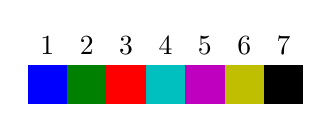
\begin{tikzpicture}[scale=0.5]
        \foreach \x/\c in {1/bb, 2/gg, 3/rr, 4/cc, 5/mm, 6/yy, 7/kk} {
            \fill[\c] (\x, 0) rectangle ++(1,1);
            \path (\x,1) ++ (right:0.5) node[above] {\x};
        };
    \end{tikzpicture}
    \caption{Color order for sweep plots in the report.}
    \label{fig:colororder}
\end{figure}

When two-port S-parameter measurements are mentioned in the report, port 1 is always the top-antenna and port 2 is the side-antenna unless otherwise noted.

